\newpage
\section{Strahlenteiler und $\frac{\lambda}{2}$ Plättchen}
\textbf{Wofür werden im Versuch zwei Strahlenteilerwürfel benötigt, die polarisierend sind? 
Wozu wird das $\frac{\lambda}{2}$ Plättchen und das Filterrad gebraucht?}\\
Mithilfe eines Strahlteilers kann man, wie es der Name bereits verrät, 
einen einzelnen Strahl in zwei Teilstrahlen aufteilen.\\
In der folgenden Abbildung \ref{fig:Strahlenteiler} ist dies schematisch aufskizziert:
\begin{figure}[h]
    \centering
    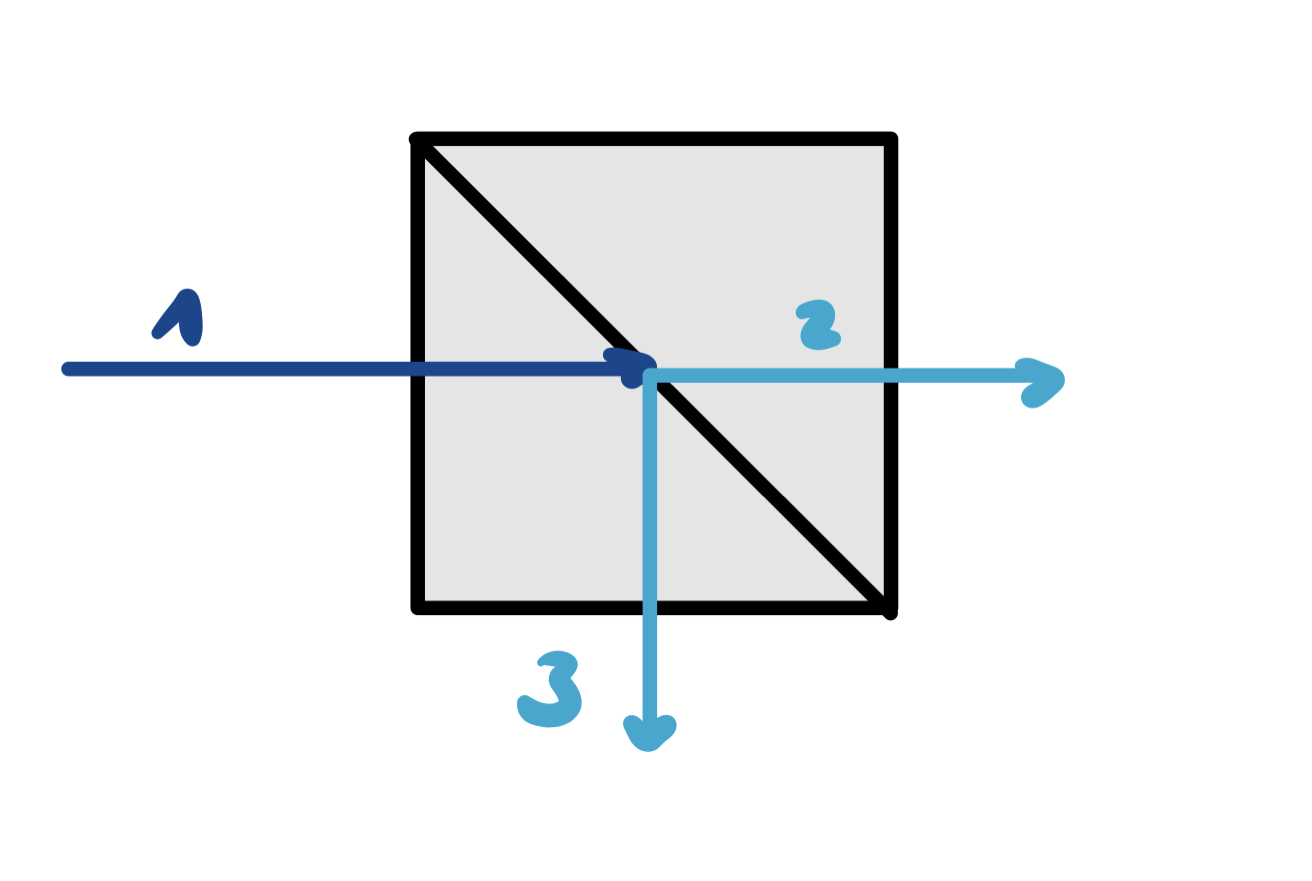
\includegraphics[scale=0.1]{Bilder/FzV/Strahlenteiler.jpg}
    \caption{Schematische Skizze eines Strahlenteilerwürfel}
    \label{fig:Strahlenteiler}
   \end{figure}\\
Bei dem Spezialfall \textit{polarisierenden Strahlteilerwürfel} ist das
Teilungsverhältnis abhägig vom Polaristationswinkel des einfallenden Lichts. \\
Alle Strahlenteile einer Polarisationsrichtung werden am Strahlteiler transmittiert, 
die restlichen Strahlanteile werden senkrecht zur Einfallsebene reflektiert.\citep[vgl.][]{Strahlteiler}\\
In unserem Versuch wird ein solcher Strahlteiler genutzt, um die Intensitäten 
des Pump- bzw. Probestrahls einzustellen zu können.\\\\
Das $\frac{\lambda}{2}$ Plättchen oder auch Verzögerungsplatte ist ein optisches
Bauelement, welches die Polarisation einer elektromagnetischen Welle ändern kann. 
Das heißt in unserem Versuch sorgt das $\frac{\lambda}{2}$ Plättchen zusammen mit 
einem linearen Polarisator dafür das der eintreffende Strahl linear polarisiert wird. 
Zusätzlich sorgt das Plättchen für einen Phasensprung um $\pi$. Dies hat zur Folge, dass 
die Polarisationsrichtung nach dem Auftreffen auf das Plättchen um 90° gedreht ist, im 
Vergleich zu vor dem Eintritt in das Plättchen.\citep[vgl.][]{Platte}\\
Mithilfe dem Filterrads lassen sich die Intensitäten einstellen und anpassen.

\section{Hyperfeinstrukturkonstante und -übergänge}
\textbf{Wie kann man aus den gewonnen Daten die Hyperfeinstrukturkonstanten berechenen?
Welche Hyperfeinübergänge sind im Spektrum zu erwarten?}\\
Im Versuch werden die Absorptionsspektren der Rubidiumisotrope gemessen. 
Mithilfe der gemessenen Absorptionslinien lassen sich Aussagen über die
Absorptionsenergien für die Übergänge treffen. Die entsprechende Energie 
ist wie folgt definiert:
\begin{equation}
    \Delta E_{HFS} = \frac{a}{2}[F(F+1)-J(J+1)-I(I+1)]
\end{equation}
Wobei F für den Gesamtdrehimpuls, J für den Gesamtdrehimpuls der Hülle und I für den Kernspin steht. \\
Diese Komponenten sind bereits bekannt und so fehlt nur noch a.\\
a ist die sogenannte Hyperfeinstrukturkonstante und ist wie folgt definiert:
\begin{equation}
    a = \frac{g_I \cdot \mu_k}{\sqrt{J(J+1)}}
\end{equation}
Hierbei wird $g_I$ als Landé-Faktor bezeichnet und $\mu_k$ steht für das Kernmagneton.\\
Das Kernmagneton wird wie folgt berechnet und $m_p$ steht hierbei für die Protonenmasse:
\begin{equation*}
    \mu_k = \frac{e \cdot \hbar}{2 m_p} = 5,05783 \cdot 10^{-27} \frac{J}{T}
\end{equation*}
\citep[vgl.][]{Kohler}\\
Die folgenden Graphen zeigen die erlaubten Hyperfeinübergänge der Isotrope \ce{^{85}Rb} 
und \ce{^{87}Rb} für die beiden möglichen D-Linien \citep[entnommen][]{AnhangA, AnhangB}.\\
Hierbei wurden die allgemein gültigen Auswahlregeln mitberücksichtigt und die möglichen Übergänge 
eingezeichnet:
\begin{align*}
    \Delta L &= \pm 1\\
    \Delta I &= 0, \pm 1\\
    \Delta J &= 0, \pm 1\\
    \Delta F &= 0, \pm 1\\
\end{align*}
\begin{figure}[h]
    \centering
    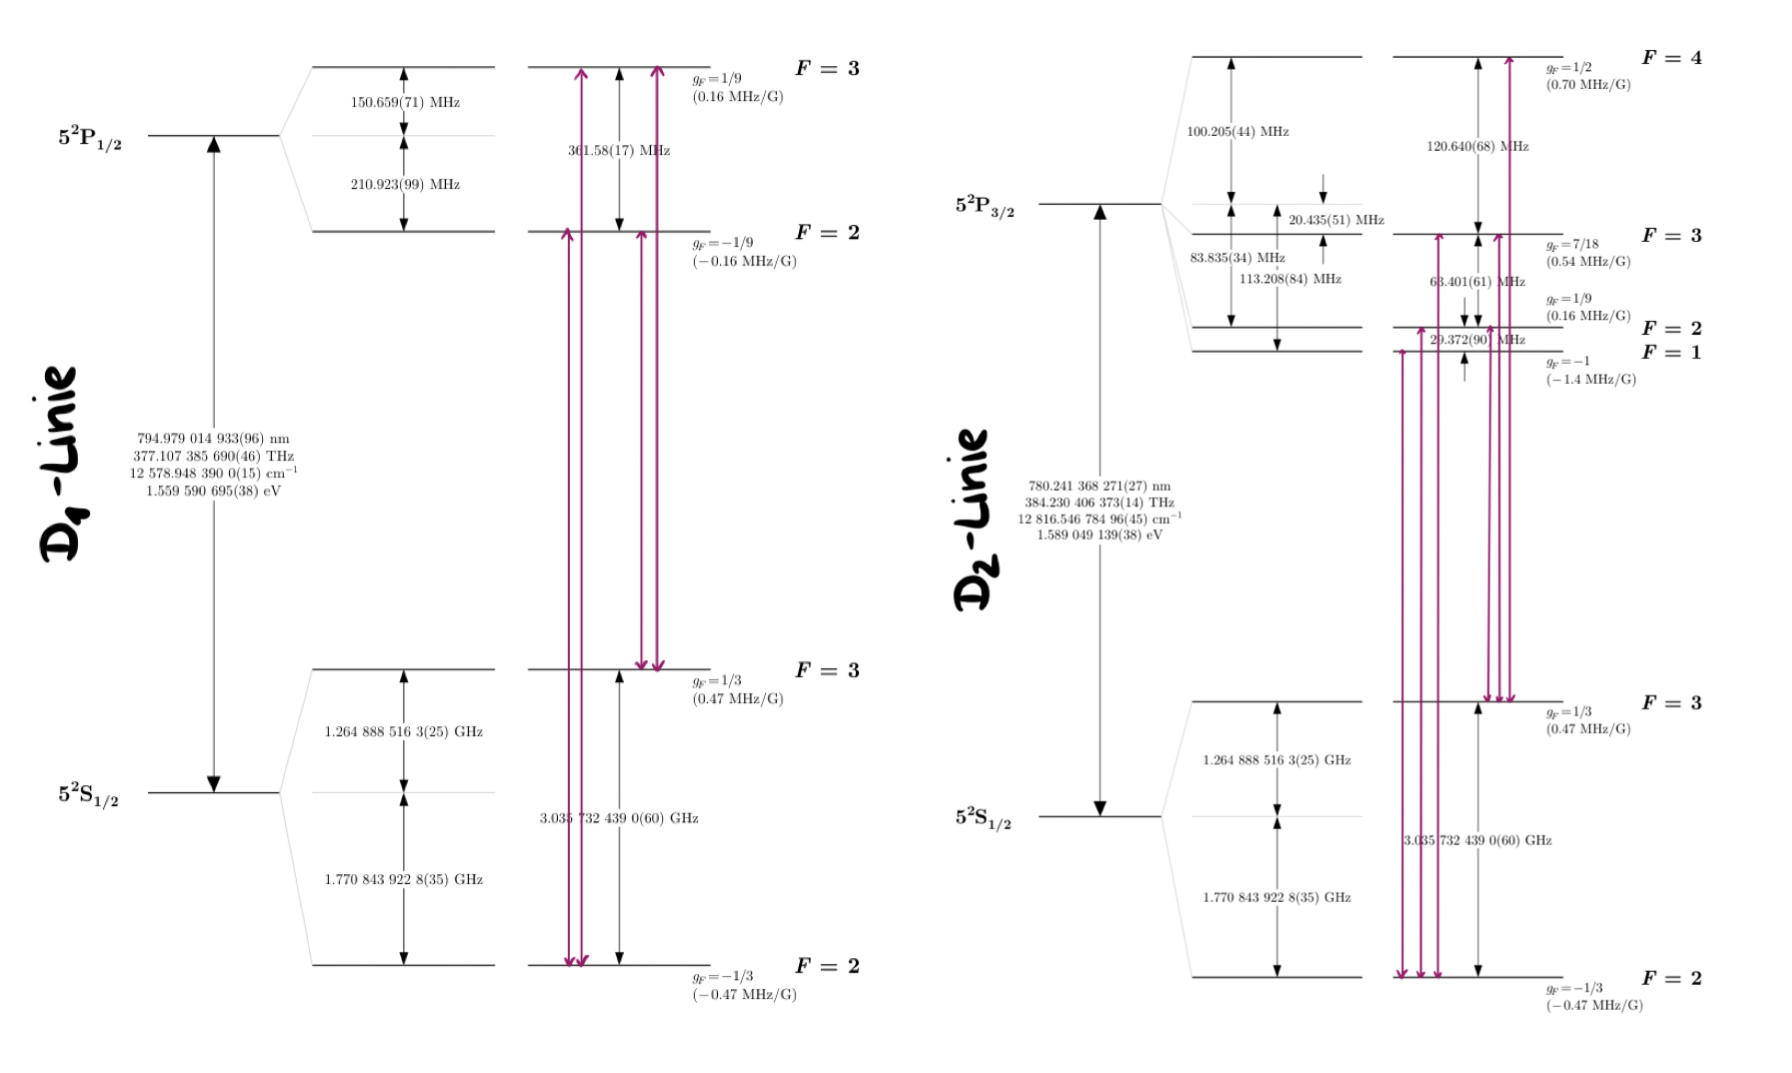
\includegraphics[scale=0.25]{Bilder/FzV/Hyp85.jpg}
    \caption{Übergänge der D1- bzw. D2-Linie von \ce{^{85}Rb}}
   \end{figure}\\
   \begin{figure}[h]
    \centering
    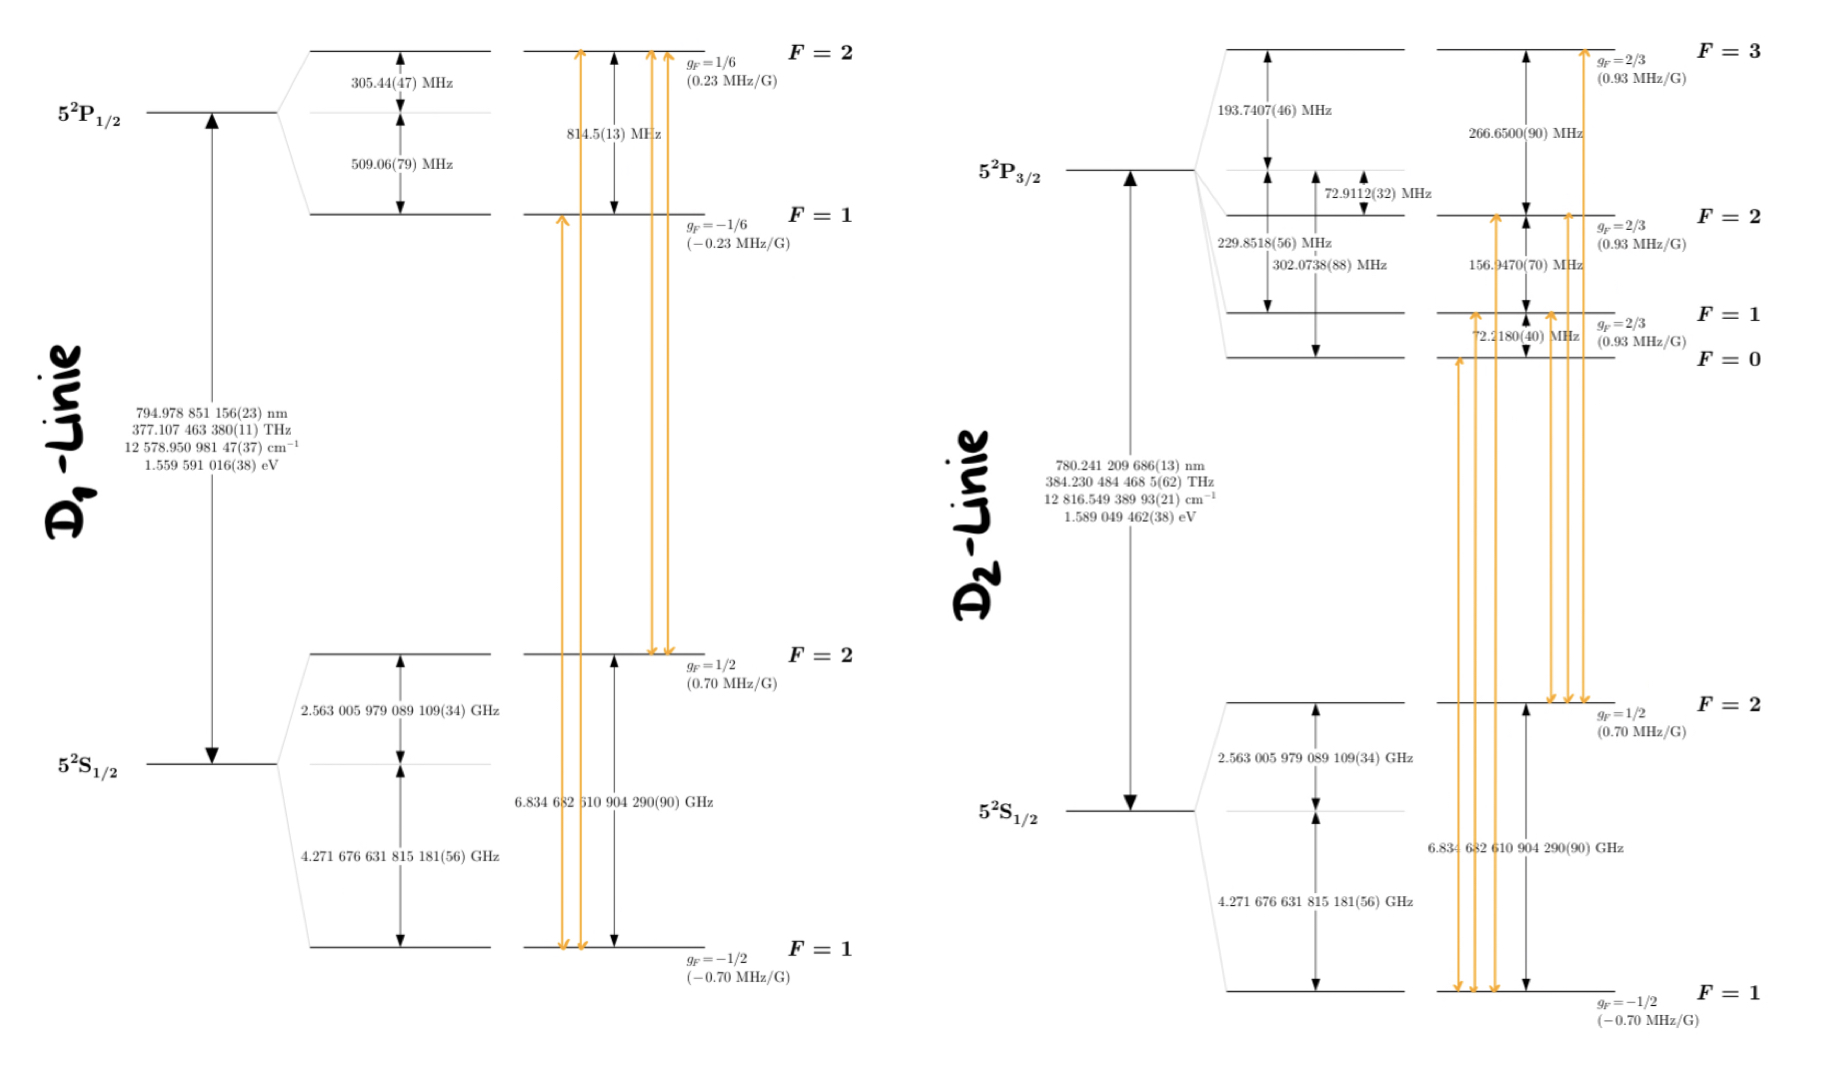
\includegraphics[scale=0.25]{Bilder/FzV/Hyp87.jpg}
    \caption{Übergänge der D1- bzw. D2-Linie von \ce{^{87}Rb}}
   \end{figure}\\
